%!TEX root = ../thesis.tex
\newchap{Semileptonic diTop decays}\label{sec:Events}
\vspace{-1cm}
\minitoc


\section{Event signatures}
In this chapter, we will name "signal" or "cb events" the $\ttbar \to b\ell\nu\: bcb$ process, and "background" everything else.\\
\\
The final state of a signal event consists of one muon or electron, three b jets, one c jet, and some missing energy due to the presence of the neutrino.\\
The invariant mass of one b jet and the c jet should match the mass of the \PW boson, and, adding another b jet, should match the mass of the top quark.\\
This final state can be mimicked by the following processes.
\begin{itemize}
    \item Semileptonic $\ttbar$ ($\ttbar\to b\ell\nu \: bq\bar{q}$): if one or more jets are mistagged or there are additional heavy flavor jets.\\
    The production of additional heavy-flavor jets is highly suppressed so, this background depends mainly on the b/c tagging capabilities of the experiment.
    \item Dileptonic $\ttbar$ ($\ttbar \to b\bar{\ell}\nu \: \bar{b}\ell\bar{\nu}$): the presence of two leptons in the final states increase the trigger probability, while the two missing jets can be originated from additional jets produced by initial state radiation (ISR) of final state radiation (FSR), or from the leptons.
    \item Dihadronic $\ttbar$ ($\ttbar \to b\bar{q}q \: \bar{b}q\bar{q}$): the missing lepton can be originated by the semileptonic decay of a meson in the jet if it passes the isolation selections, and the missing b jet can be obtained by mistagging or by additional heavy flavor jets.
    \item W+jets $(\PW \to \ell \nu)$: This process is the one with the largest cross-section but the lack of three b jets and one c jets suppress it significantly.
    \item WW+jets: the semileptonic decay of \PW pairs produced directly by $pp$ collision, in association with two other b jets, has the same signal signature. Another difference with the signal is the mismatch of the invariant mass of 3 jets with the top mass, which, however, is difficult to exploit due to the combinatorial ambiguities and the low tri-jet mass resolution.  
    \item $t\PW+\text{jets}$: it is similar to the $\PW \PW + \text{jets}$ process, with the difference that only one additional b jet instead of two is required to match the signal signature.
    \item $tq$ (t-channel): if the top quark decays into a lepton. There are two missing b jets and, if the quark is not a charm quark, also a c jet.
\end{itemize}
The production cross-sections of these processes  at $\sqrt{s}=13\TeV$ with $pp$ collisions are reported in Tab.\ref{tab:cross}


\begin{table}[H]
    \centering
    \fontsize{9.2pt}{9.2pt}\selectfont
    \begin{tabular}{l|cccc|c|c|c|c}
        \toprule
          \multicolumn{1}{c|}{$\mathbf{pp\to}$}&\multicolumn{4}{c|}{$ \mathbf{t\bar{t}}$}&  $ \mathbf{W}$& $ \mathbf{WW}$ & $ \mathbf{tW}$& $ \mathbf{tq}$\\
          &&  &  &  &  &   & & (t-channel)\\
          \midrule
          \multicolumn{1}{c|}{$\mathbf{\sigma (pb)}$}&\multicolumn{4}{c|}{\multirow{2}{*}{$832$}}& \multirow{2}{*}{$59100$} & \multirow{2}{*}{$118$} &  \multirow{2}{*}{79}& \multirow{2}{*}{214} \\
          \multicolumn{1}{c|}{$(13\TeV)$}& &  & & &  &&&\\
          \midrule
          &signal&  semiLept&  diLept&  diHad& Lept &  semiLept & semiLept& Lept\\
          &$(b\ell \nu\: bcb)$&$(b\ell \nu\: b\bar{q}q)$&$(b\bar{\ell} \nu\: \bar{b}\ell \bar{\nu})$&$(\bar{b}\bar{q}q\: b\bar{q}q)$&$(\ell \nu)$&$(\ell \nu \: q\bar{q})$& $(b\ell\nu q \bar{q})$&$(b\ell\nu \: q)$\\
          \midrule
          $\mathcal{BR}$& $3.7 \cdot 10^{-4}$   & 0.439 & 0.106 & 0.455 & 0.326 & 0.106 & 0.439 & 0.326\\
          $ \mathcal{BR}\cdot\mathbf{\sigma} (pb)$& 0.307 & 365 & 88 & 379 & 19200 & 12.5 & 34.7& 69.8 \\
          $\mathcal{BR}\cdot\mathcal{L}_I\mathbf{\sigma} $&$4.2 \cdot 10^4$& $5.0 \cdot 10^7$ &  $1.2 \cdot 10^7$&$5.2 \cdot 10^7$  &  $2.6 \cdot 10^9$ & $1.7 \cdot 10^6$  & $4.8 \cdot 10^6$& $9.6 \cdot 10^{6}$\\
          \bottomrule
    \end{tabular}
    \vspace{0.2cm}
    \caption{Production cross-sections of signal and backgrounds at $\sqrt{s}=13\TeV$. In the first row, there are the production cross-sections from pp collisions at $13 \TeV$, in the following rows there are the respective branching fractions of the different final states, the cross-section of the respective final states, and the total number of events expected in all the Run2, with a total integrated luminosity of $\mathcal{L}_I=138 {fb}^{-1}$}
    \label{tab:cross}
\end{table}

\iffalse
\begin{figure}[H]
    \vspace{-0.5cm}
     \centering
     \begin{subfigure}{0.48\linewidth}
         \centering
         \includegraphics[width=\linewidth]{fig//chap07-selection/LHE_Nb.png}
         \caption{b quark}

     \end{subfigure}
     \hfill
     \begin{subfigure}{0.48\linewidth}
         \centering
        \includegraphics[width=\linewidth]{fig//chap07-selection/LHE_Nc.png}
         \caption{c quark}
     \end{subfigure}
        \caption{Stacked histogram of the number of c and b quarks for each sample at the parton level.}
        \label{fig:LHE_flav}
\end{figure}
\fi

\paragraph*{Analysis strategy}
In the following sections, the selection criteria for physics objects and events are described, defining different signal regions for $\ell=\mu,e$.
Therefore, after reconstructing the kinematics of the events, the signal extraction is performed through a template fit on a NN score, by exploiting multivariate analysis techniques, and also studying the relevant signatures of the events.\\
This work will be conducted only on MC simulations and the observed data will be replaced by the Asimov dataset.



\section{Simulation samples}
The generators that were used to build the MC samples are \MADGRAPH 5 (at the leading order (LO)) and aMC@NLO and \POWHEG 2 (at the next-to-leading order (NLO), including virtual corrections). In all samples, the used PDF set is NNPDF3.1 NNLO and the mass of the top quark is set to 172.5\GeV. The hadronization is handled by \PYTHIA8 exploiting the Lung string model with the \texttt{TuneCP5} set of tuning parameters \cite{Sirunyan2020ExtractionMeasurements}: the $\alpha_S$ value used for the simulation of the multiparton interaction (MPI)\footnote{The MPI are additional soft or semi-hard parton–parton scatterings that occur within the same hadron-hadron collision.}, hard scattering, and FSR and ISR contributions is equal to 0.118 and it runs according to an NLO evolution.
For each sample, a different number of additional partons is generated to include FSR and ISR contributions and virtual corrections at NLO.
\\
After the parton shower evolution, the final jet clusters are matched with the partons obtained from the matrix element calculations and if the match is found, the event is removed to avoid the double counting\footnote{This procedure is called "Jet matching"}.
\\
\\
The reconstruction and the calibration are performed with the \textit{Ultra Legacy 18} (UL18) setting, which reproduces the state of the detector in 2018.\\
The used samples are NanoAOD files \cite{Liu2020TheCMS}, a lightweight data format that consists only of flat ROOT NTuple.
\\
A comparison of all the used samples is reported in Table \ref{tab:samples}.
\begin{table}[H]
    
    \centering
    \fontsize{10.5pt}{10.5pt}\selectfont
    \begin{tabular*}{\linewidth}{@{\extracolsep{\fill}}cccc|c}
    \toprule
    \multirow{2}{*}{\textbf{Dataset}}&\multirow{2}{*}{\textbf{Generator}} & \textbf{Additional} & \multirow{2}{*}{$\mathcal{L}_I^{\text{MC}}/\mathcal{L}_I^{\text{RunII}}$}& \multirow{2}{*}{\textbf{Label}}  \\
    &&\textbf{Partons}& &\\
    \midrule
    \ttbar signal& \MADGRAPH (LO) & \multirow{2}{*}{3} &\multirow{2}{*}{76.5}& $\ell=\mu,e,\tau$  \\
    $(b\ell\nu \: bcb)$ &+\MADSPIN & && signal(Mu,Ele,Tau) \\    
    \midrule
    \ttbar semiLept&\multirow{2}{*}{\POWHEG (NLO)} &\multirow{2}{*}{1}&\multirow{2}{*}{2.24} & $\ell=\mu,e,\tau$   \\
    $(b\ell\nu \: bqq)$ && && TTsemiLept(Mu,Ele,Tau)\\  
    \midrule
    \ttbar diLept&\multirow{2}{*}{\POWHEG (NLO)}  &\multirow{2}{*}{1}&\multirow{2}{*}{1.71} & \multirow{2}{*}{TTdiLept}\\
    $(b\bar{\ell}\nu \:\bar{b}\ell\bar{\nu})$&& &\\
    \midrule
    \ttbar diHad&\multirow{2}{*}{\POWHEG (NLO)} &\multirow{2}{*}{1}&\multirow{2}{*}{0.87} &\multirow{2}{*}{TTdiHad}\\
    $(bq\bar{q}\: \bar{b}q\bar{q})$&& &\\
    \midrule
    W+jets& \MADGRAPH (LO) &\multirow{2}{*}{4}&\multirow{2}{*}{0.02} &\multirow{2}{*}{WJets}\\
    $(W\to\ell\nu)$&+\MADSPIN &&\\
    \midrule
    WW+jets&aMC@NLO (NLO) & \multirow{2}{*}{1} & \multirow{2}{*}{0.56}& \multirow{2}{*}{WWJets}\\
    $\ell \nu \: q\bar{q}$&+\MADSPIN&&\\
    \midrule
    t\PW & \multirow{2}{*}{\POWHEG (NLO)} & \multirow{2}{*}{1} & \multirow{2}{*}{0.16} & \multirow{2}{*}{tW}\\
    $(b\ell\nu q\bar{q})$&&&&\\
    \midrule
    tq (t-channel) & \multirow{2}{*}{\POWHEG (NLO)} &  \multirow{2}{*}{1} & \multirow{2}{*}{0.11} & \multirow{2}{*}{tq}\\
    $b\ell\nu q$&&&&\\

    \bottomrule
    \end{tabular*}
    \caption{MC samples used in this work along with the respective generator used, the number of additional partons set in the generator, and the ratio between the effective luminosity of the MC sample and the integrated luminosity of the RunII. In the "Label" column there are the names that are used as labels in the rest of the thesis.}
    \label{tab:samples}
\end{table}





Simulated events are normalized to
their expected contributions using event weights 
\begin{equation}
    w_{pe}=\frac{\mathcal{L}_I \cdot \sigma_p \cdot w_{e} }{\sum_j w_{j}}
\end{equation}

where $w_{e}$ is the event weight obtained by the product of the weights produced by the generator program with the weights obtained by the jet flavor corrections (see sec. \ref{sec:jet})   

\section{Physics objects selections}
As already said, the idea of the analysis is to focus on semileptonic (SL) decay to exploit the lepton as a probe, so we are interested in selecting one prompt lepton, along with four jets.
The selection of physics objects is crucial to reject non-prompt leptons that can originate from the semileptonic decays of mesons and jets that can originate from prompt leptons or pile-up.\\
\\
The objects taken into consideration are Particle Flow candidates (see sec. \ref{sec:PF}) and the applied selection cuts are the working points (WP) recommended by the CMS Physics Object Groups (POG).\\
Since the signal cross-section is just $\sigma_{\text{signal}}\sim 0.3 pb$, the requirements will be minimal to preserve the statistics. 
\subsection{Muons}
\paragraph*{Identification}
The selected muons are PF candidates reconstructed as \emph{Loose Muons}, \ie muon candidates that are reconstructed either as a global muon or as an arbitrated tracker muon (aTk Muons)\footnotemark.\\
Furthermore, the selected muons must be in the coverage of the tracker $|\eta|<2.4$, and its transverse momentum has to be $p_T>26\GeV$ to pass the HLT single muon trigger.
\paragraph*{Isolation}
To select prompt muons from the \PW decay, the particle flow isolation criteria are applied.
\footnotetext{Arbitration is the pattern recognition process that assigns each segment uniquely to a single tracker muon.}
\\
The PF isolation is the scalar sum of the transverse momentum of all the charged particles, neutral hadrons, and  photons inside a cone of radius $\Delta R<0.4$ around the selected muon, subtracting the contributions that arise from pile-up effects \cite{2018MuonData}.    
\begin{equation}
    \text{Iso}_\mu = \left(\sum_{\text{charged}} p_T+\max\left(0,\sum_{\text{neutral}}E_T+\sum_{\text{photons}}E_T-\sum_{\text{PileUp}}p_T/2\right)\right)\bigg/p_T(\mu)
\end{equation}
The selected working point is the \emph{Loose PF Isolation}: $\text{Iso}_\mu<0.25$, which leads to a muon selection efficiency of $\sim 98\%$ evaluated on $Z \to \mu \bar{\mu}$ samples.






\subsection{Electrons}
The selection of electron candidates follows the same principles as the muon selections.
They are required to be into the tracker coverage $|\eta|<2.4$ and its momentum has to be $p_T>30$.\\
\\
The identification and isolation of the electron are based on the \emph{medium} working point of \textit{Fall17IsoV2} \cite{2018ElectronConference}, a BDT model which assigns a score to the identification and isolation of the electron, taking as input informations about tracks, calo-clusters, shower shape, the amount of collinear radiation to the electron track, and the PF isolation.\\
\\
The MVA ID is trained on DrellYan+Jets MC samples, with prompt electrons as signal and unmatched plus non-prompt electrons as background, ignoring electrons from tau decays.\\
\\
The medium working point has an overall signal efficiency of $\sim 90\%$ and a background rejection efficiency $>98.5\%$.
\subsection{Jets}\label{sec:jet}
The jets taken into consideration are the PF AK4 Jet candidates in the calorimeter coverage $|\eta|<4.8$ and with $p_T>20\GeV$.

\paragraph*{Jet energy corrections}
The jet momentum and the jet mass resolution are lower in the data with respect to the simulation. To replicate the resolution observed in the data, the jets' four vectors are rescaled in a procedure called \emph{smearing} \cite{2021Jet13TeV}:\\
if a reconstructed jet and a jet at the generator level (GenJet) are matched through the relation $\Delta R(\text{Jet,GenJet})<0.2$ and $|p_T-p_T^{\text{Gen}}|<3\sigma p_T$, the jet four-vector is scaled by a factor
\begin{equation}
    f=1+\textit{SF}\:\frac{p_T-p_T^{\text{Gen}}}{p_T}
\end{equation}
otherwise, a random Gaussian smearing is applied.\\
$\sigma$ is the jet energy resolution measured with data, and SF are the scale factors provided by the JETMET POG, that depend on the $\eta$ region in which the jet belongs.

\paragraph*{Flavor tagging corrections}
The distribution shape of the \DeepJet discriminator is another element that shows discrepancies between data and simulated samples.\\
To improve the agreement between MC simulations and data, simulated events are reweighted, and, for each correction, the event weight is the product of all the weights.\\
For each selected jet, a weight is applied to it, setting the event weight to the product of all the jet-level weights.
\\
\\
In this work, the applied corrections are the ones related to the b tagging and to the c tagging.\\
These scale factors are computed through an iterative tag-and-probe procedure \cite{2021B-tagging2018.}, in different bins of $\eta$,$p_T$, and \DeepJet score to compute simultaneously SF for both heavy and light flavor jets.
\begin{itemize}
    \item For heavy-flavor jets, dileptonic $\ttbar$ events are exploited, using one b jet that passes the medium working point as a tag and the second b jet as a probe.
    \item For light jets, Z+jets dileptonic samples are used, using a b tag loose working point as a veto to select the tag jet.
\end{itemize}
The distribution of the \DeepJet score of the probe jets in MC samples is normalized to match the distribution observed in the data subtracting the contribution from jets of opposite flavour class.
\begin{equation}
    \text{SF}_{\text{HF/LF}} (\DeepJet,p_T,\eta)=\frac{\text{Data}-\text{MC}_{\neg(\text{HF/LF})}}{\text{MC}_{\text{HF/LF}}}
\end{equation}
The SFs are evaluated iteratively until they converge
\begin{equation}
    \text{SF}_{\text{HF/LF}}^{i+1} =\dfrac{\text{Data}-\text{SF}_{\neg (\text{HF/LF)}}^{i} \text{MC}_{\neg(\text{HF/LF})}}{\text{MC}_{\text{HF/LF}}}
\end{equation}
The procedure to obtain SFs related to the c-tagging is similar, using W+c samples, but for them, the binning depends both on the CvB and CvL discriminators.



\paragraph*{Identification}
The jet identification is based on the \emph{Tight jetID} that imposes different requirements on the substructure of the jets in different $|\eta|$ regions.\\
The requirements are listed in Tab.\ref{tab:jet_id}

\begin{table}[H]
    \centering
    \fontsize{11pt}{11pt}\selectfont
    \begin{tabular}{l|c|c|c|c}
        \toprule
         \multicolumn{1}{c|}{$\bm{|\eta|\in}$}&  $[0,2.6]$& $[2.6,2.7]$ & $[2.7,3.0]$ & $[3.0,5.0]$\\
         \midrule
         \textbf{Neutral Hadron Fraction} & $<0.90$ &  $<0.90$ & - & $>0.20$\\
         \midrule
         \textbf{Neutral EM Fraction} & $<0.90$ & $<0.99$ & $\in[0.02,99]$ & $<0.90$\\
         \midrule
         \textbf{Number of Constituents } & $>1$ & - & - &  -\\
         \midrule
         \textbf{Charged Hadron Fraction} & $>0$ & - & - & -\\
         \midrule
         \textbf{Charged Multiplicity} & $>0$ & $>0$ & - & -\\
         \midrule
         \textbf{Number of Neutral Particles}& - & - & $>2$ & $>10$\\
         \bottomrule
    \end{tabular}
    \caption{Tight jet identification requirements.}
    \label{tab:jet_id}
\end{table}
The efficiency of the tight Id working point is $\epsilon>99\%$, whereas the background rejection is $>98\%$. 
\paragraph*{Isolation} 
To avoid the misidentification of the lepton as a jet originated from a quark parton, a simple $\Delta R$ matching is performed. If the jet axis and the leading lepton are separated less than $\Delta R<0.4$, the jet is removed. 

\paragraph*{Pile-up rejection}
The identification of jets from pile-up relies on three types of properties of the jets:
\begin{itemize}
    \item  In the tracker acceptance, the tracks associated with the jets can be used to match the jet with the primary interaction vertex.
    \item The shape of the calorimetric deposit is different in case of overlap of multiple interactions.
    \newpage
    \item The objects' multiplicity.
\end{itemize}


\begin{minipage}{\linewidth}
    \begin{minipage}{0.4\linewidth}
        The identification of jet from pile-up is done exploiting the \emph{Jet puId},
        a BDT model score \cite{CMSCollaboration2020PileupData}. Its inputs are listed in Tab \ref{tab:puId_inputs}.\\
        \\
        This BDT is trained on DrellYan+Jets MC samples with jets of $p_T<50\GeV$, where there is the highest composition of PU jets.\\
        \\
        The chosen working point is the \emph{Loose puId}, which corresponds to 99\%  efficiency for prompt jets with $|\eta| < 2.5$ and 95\% efficiency for prompt jets with $|\eta| > 2.5$.
    \end{minipage}
    \hfill
    \begin{minipage}{0.55\linewidth}
        \vspace{-1.5cm}
    
        \begin{table}[H]
        \centering
        \fontsize{9.2pt}{9.2pt}\selectfont
        \begin{tabular}{|l|p{6cm}|}
        \hline
        \textbf{Variable} & \textbf{Description} \\
        \hline
        \textbf{nvtx} & Number of primary vertices \\
        \hline
        \textbf{beta} & Fraction of jet tracks associated with the primary vertex \\
        \hline
        \textbf{dR2Mean} & $p^2$-weighted average square distance of jet constituents from the jet axis \\
        \hline
        \textbf{frac01} & Fraction of constituents' $p_T$ contained in the region $\Delta R < 0.1$ around the jet axis \\
        \hline
        \textbf{frac02} & Fraction of constituents' $p_T$ contained in the ring $0.1 < \Delta R < 0.2$ around the jet axis \\
        \hline
        \textbf{frac03} & Fraction of constituents' $p_T$ contained in the ring $0.2 < \Delta R < 0.3$ around the jet axis \\
        \hline
        \textbf{frac04} & Fraction of constituents' $p_T$ contained in the ring $0.3 < \Delta R < 0.4$ around the jet axis \\
        \hline
        \textbf{jetR} & Fraction of jet $p_T$ carried by the leading constituent \\
        \hline
        \textbf{jetRchg} & Fraction of jet $p_T$ carried by the leading charged constituent \\
        \hline
        \textbf{majW} & Major axis of the jet ellipsoid in the $\eta - \phi$ plane \\
        \hline
        \textbf{minW} & Minor axis of the jet ellipsoid in the $\eta - \phi$ plane \\
        \hline
        \textbf{nCharged} & Number of charged constituents \\
        \hline
        \textbf{nParticles} & Number of constituents \\
        \hline
        \textbf{ptD} & $p_T$-weighted average $p_T$ of constituents \\
        \hline
        \textbf{pull} & Magnitude of the pull vector \\
        \hline
        \end{tabular}
        \caption{Inputs of the BDT Jet\_puId model.}
        \label{tab:puId_inputs}
        \end{table}
        
    \end{minipage}
    
\end{minipage}

\begin{center}
    \vspace{1.5cm}
    \fontsize{14}{14}\selectfont
    \textbf{Summary Jets}
\end{center}

\begin{minipage}{\linewidth}
\begin{minipage}{0.53\linewidth}
      \begin{figure}[H]
            \centering
            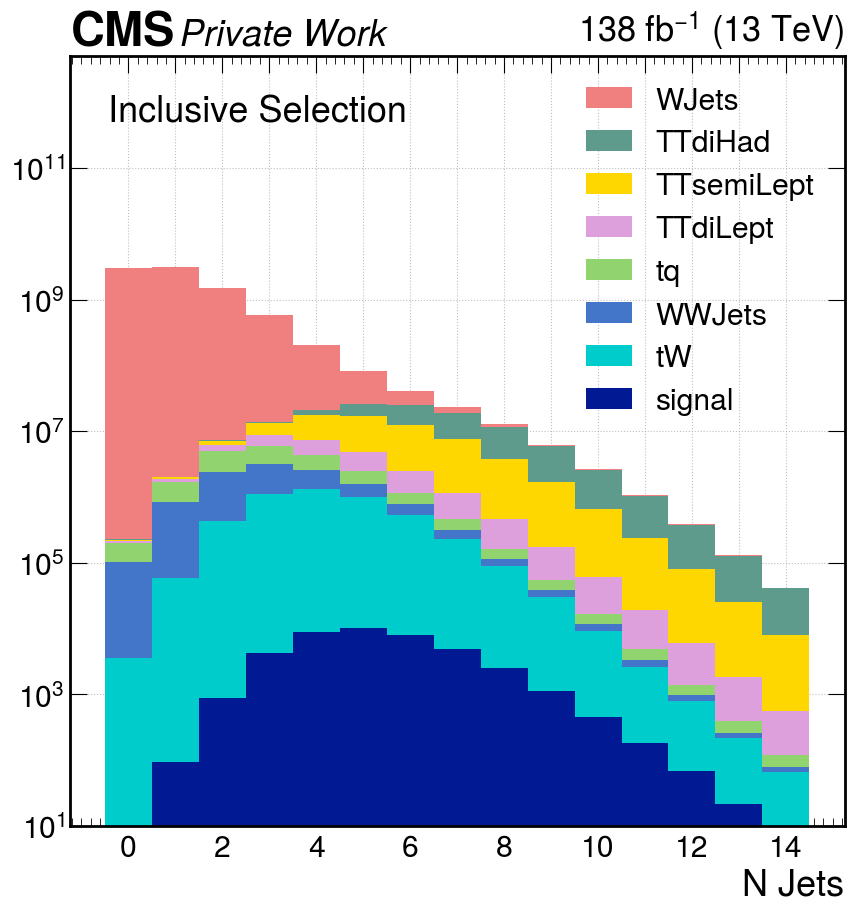
\includegraphics[width=1\linewidth]{fig//chap07-selection/nJet.png}
            \caption{Distribution on the number of Jets per event per process after the object selection.}
            \label{fig:n_jet}
        \end{figure}
\end{minipage}
\hfill
\begin{minipage}{0.46\linewidth}
\vspace{-1.25cm}
\begin{table}[H]
    \centering
    \begin{tabular}{c|c}
        \toprule
        \multicolumn{2}{c}{\textbf{Jets}}\\
        \midrule
        \midrule
        
        $\mathbf{p_T}$& $>20 \GeV$\\
        \midrule
        $\bm{|\eta|}$& $<4.8$ \\
        \midrule
        \textbf{Identification} & Tight\\
        \midrule
        \multirow{2}{*}{\textbf{Isolation}} & Lead. Lept. \\
        &$\Delta R>0.4$ matching\\
        \midrule
        \textbf{Pile-up Id} & Loose  $(\epsilon\sim99\%)$ \\
        \bottomrule
    \end{tabular}
    \caption{Jets selection cuts.}
\end{table}
\end{minipage}   
\end{minipage}

\newpage
\begin{center}
    \vspace{1cm}
    \fontsize{14}{14}\selectfont
    \textbf{Summary Muons}
\end{center}
\begin{minipage}{\linewidth}
\begin{minipage}{0.46\linewidth}
\vspace{-1.25cm}
        \begin{table}[H]
        \centering
        %\fontsize{10.2pt}{10.2pt}\selectfont
        \begin{tabular}{c|c}
            \toprule
            \multicolumn{2}{c}{\textbf{Muons}}\\
            \midrule
            \midrule
            \textbf{Muon} & Loose\\
            \textbf{Identification}& (Global/aTk Muon)\\
            \midrule
            $\mathbf{p_T}$& $>26 \GeV$\\
            \midrule
            $\bm{|\eta|}$& $<2.4$ \\
            \midrule
            \multirow{2}{*}{\textbf{PF Isolation}}&Loose\\
            &$(\text{Iso}_\mu<0.25)$\\
            \bottomrule
        \end{tabular}
        \caption{Muons selection cuts.}
    \end{table}
\end{minipage}
\hfill
\begin{minipage}{0.53\linewidth}
      \begin{figure}[H]
            \centering
            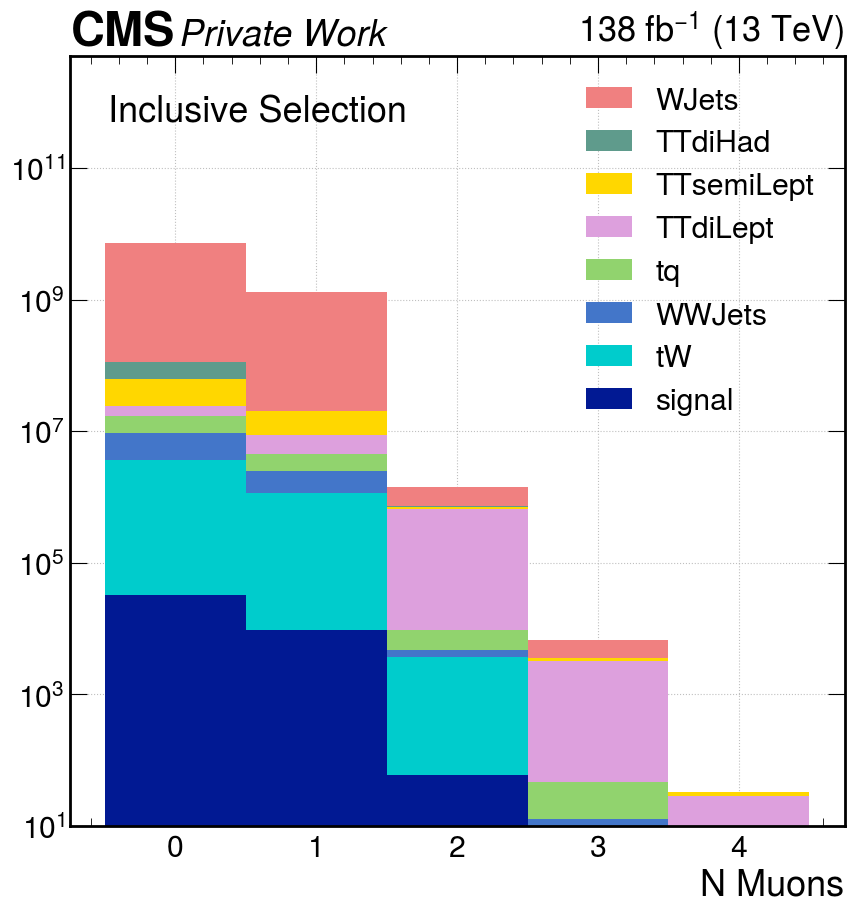
\includegraphics[width=1\linewidth]{fig//chap07-selection/nMuons.png}
            \caption{Distribution on the number of Muons per event per process after the object selection.}
            \label{fig:n_mu}
        \end{figure}
\end{minipage}
\end{minipage}




\begin{center}
    \vspace{1cm}
    \fontsize{14}{14}\selectfont
    \textbf{Summary Electrons}
\end{center}
\begin{minipage}{\linewidth}
    \begin{minipage}{0.53\linewidth}
        \begin{figure}[H]
            \centering
            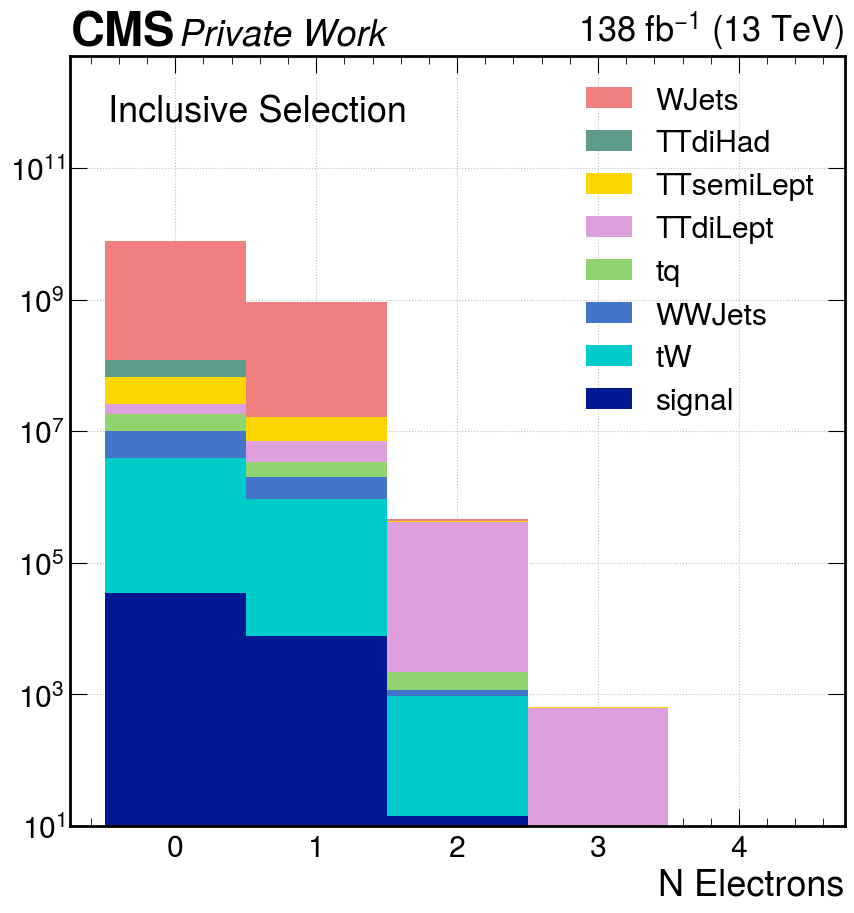
\includegraphics[width=1\linewidth]{fig//chap07-selection/nElectrons.png}
            \caption{Distribution on the number of Electrons per event per process after the object selection.}
            \label{fig:n_ele}
        \end{figure}
    \end{minipage}
    \hfill
    \begin{minipage}{0.46\linewidth}
        \vspace{-1.5cm}
        \begin{table}[H]
            \centering
            %\fontsize{13pt}{13pt}\selectfont
            \renewcommand{\arraystretch}{1.48}
            \begin{tabular}{c|c}
                \toprule
                \multicolumn{2}{c}{\textbf{Electrons}}\\
                \midrule
                \midrule
                $\mathbf{p_T}$& $>30 \GeV$\\
                \midrule
                $\bm{|\eta|}$& $<2.4$ \\
                \midrule
                \textbf{$e$ Identification}&Medium WP\\
                \textbf{+ Isolation}&Fall17IsoV2 \\
                &$(\epsilon \sim 90\%)$\\
                \bottomrule
            \end{tabular}
            \caption{Electrons selection cuts.}
        \end{table}      
    \end{minipage}
\end{minipage}

 
\newpage
\section{Event selections}
As already discussed, the chosen event selection is minimal to avoid large losses in the signal acceptance efficiency.\\ 
The signal events are targeted in two different final states, defined by the flavor of the lepton used as a probe, so, after the physics objects selection, two different channels are defined: a Muon channel that contains events with at least one selected muon, and an Electron channel that contains events with at least one selected electron.\\
An additional selection on the most b-tagged jet is imposed using the medium working point suggested by the BTag\&Vertexing (BTV) POG.\\
\\
The cumulative efficiencies of each cut are described in Tab.\ref{tab:event_selection} and the final event counts normalized with the RunII luminosity and the respective cross-sections in \Fig{fig:event_selection}
\begin{table}[H]
    \centering
    \fontsize{11.5pt}{11.5pt}\selectfont
    \begin{tabular}{l|ccc||ccc}
        \toprule
         &  \multicolumn{3}{c||}{\textbf{Muons}} &\multicolumn{3}{c}{\textbf{Electrons}} \\
         \midrule
         \midrule
         Cumulative& \multirow{2}{*}{$\bm{\geq1 \mu}$} & \multirow{2}{*}{$\bm{\geq4}$ \textbf{Jets}} & $\bm{\max({\textbf{btag}})}$& \multirow{2}{*}{$\bm{\geq1e}$} & \multirow{2}{*}{$\bm{\geq4}$ \textbf{Jets}} & $\bm{\max({\textbf{btag}})}$\\
         efficiencies&&&$\bm{>0.27}$&&&$\bm{>0.27}$\\
         \midrule
         \textbf{signalMu}& $64.1\%$ & $53.5\%$ & $51.8\%$ &0.22\% & 0.18\% & 0.16\%\\
         \midrule
         \textbf{signalEle}& 0.65\% & 0.50\% & 0.46\% & 52.3\% & 43.5\% & 42.1\% \\
         \midrule
         \textbf{signalTau}& 4.86\% & 3.95\% & 3.80\% & 3.37\% & 2.79\% & 2.70\%\\
         \midrule
         \textbf{TTsemiLeptMu}& 21.2\% & 18.0\% & 16.6\% & 0.05\% & 0.04\% & 0.03\% \\
         \midrule
         \textbf{TTsemiLeptEle}& 0.16\% & 0.13\% & 0.10\% & 17.3\% & 15.2\% & 13.9\% \\
         \midrule
         \textbf{TTsemiLeptTau}& 1.53\%  & 1.28\% & 1.16\% &1.08\% &0.94\% &0.86\%\\
         \midrule
         \textbf{TTdiLept}& 40.9\% & 27.4\% & 25.3\% & 33.8\% &22.7\% &20.9\% \\
         \midrule
         \textbf{TTdiHad}& 0.45\%  & 0.40\% & 0.31\% & 0.16\% &0.15\% &0.12\% \\
         \midrule
         \textbf{WJets Lept}& 15.0\% & 0.24\% & 0.03\% & 10.6\% & 0.20\% &0.03\%\\
         \midrule
         \textbf{WWJets SL}& 19.4\% & 5.52\% & 0.81\% & 15.3\% & 4.42\% & 0.64\% \\
         \midrule
         \textbf{tW SL}& 26.7\% & 13.4\%  & 11.2\% & 21.7\% &10.8\% &9.0\%  \\
         \midrule
         \textbf{tq Lept}& 20.5\%  & 5.13\% & 4.27\% & 15.0\% & 3.83\% &3.18\% \\
         \bottomrule
    \end{tabular}
    \caption{Cumulative efficiencies of the selections in the Muons and Electrons channel after the physics objects selection}
    \label{tab:event_selection}
\end{table}

The main background contribution in each channel is from the \ttbar semileptonic decay, that is 3 order of magnitude greater than the signal.\\
Another significant contribution is from the \ttbar dileptonic (DL) process. The contribution from the WW+Jets process is two order of magnitude smaller than \ttbar SL and \ttbar DL processes, while the remaining processes' contribution is one order of magnitude smaller than the leading backgrounds. 

\begin{figure}[H]
     \centering
     \begin{subfigure}{0.7\linewidth}
         \centering
         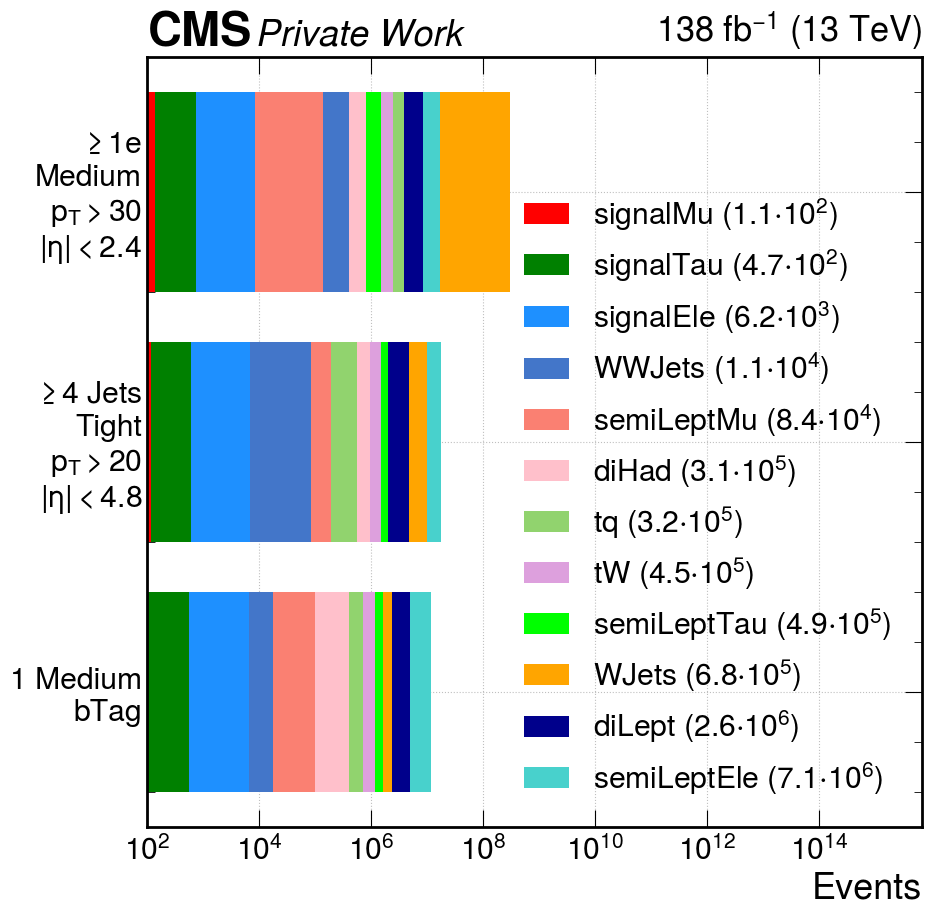
\includegraphics[width=\linewidth]{fig//chap07-selection/ele_selection.png}
         \caption{Electrons channel}

     \end{subfigure}
     
     \vspace{0.5cm}
     \begin{subfigure}{0.7\linewidth}
         \centering
        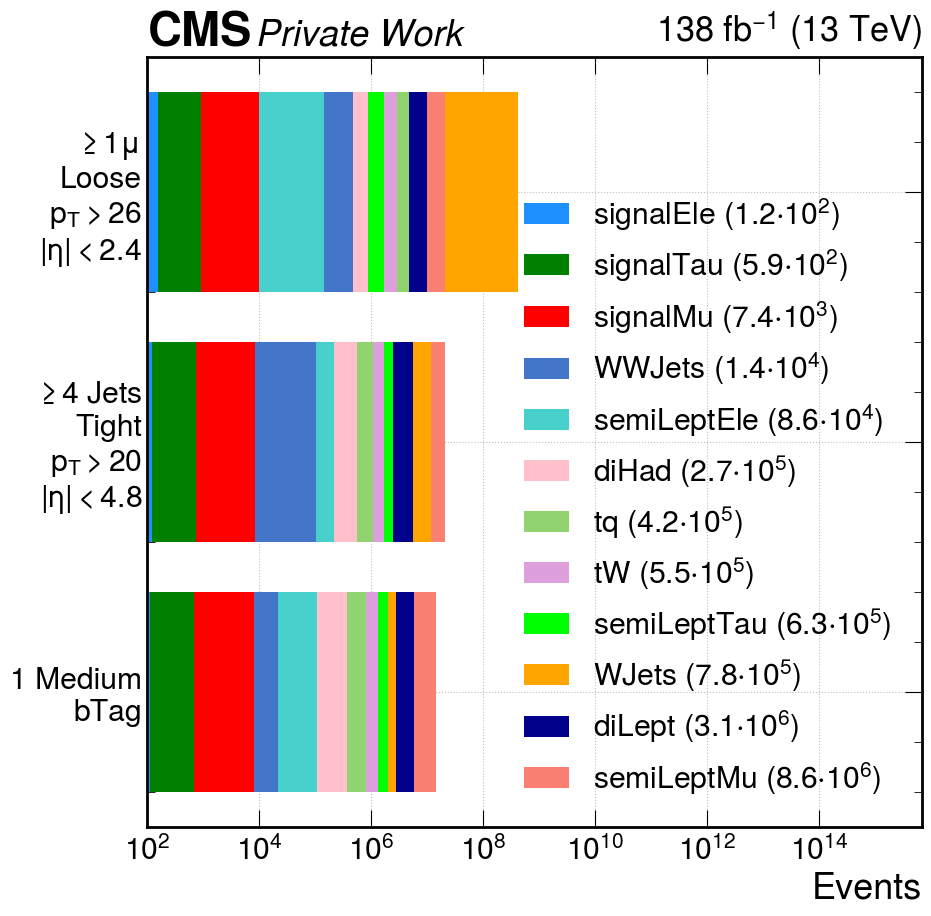
\includegraphics[width=\linewidth]{fig//chap07-selection/mu_selection.png}
         \caption{Muons channel}
     \end{subfigure}
     \vspace{0.5cm}
        \caption{Event number for each process for each cut. In the legend the final number of events for each process after the preselection is shown. The processes are ordered in their final event number.}
        \label{fig:event_selection}
\end{figure}
\TODO{PLOT: prima di event selection ma post obj selection: nJet,nMu,nEle}
\TODO{PLOT: Dopo event selection ma senza btag cut: Jet\_{pt,btag} up to 4 (linea taglio su btag leading), ctag up to 2, leading mu and ele pt}
\newpage
\section{Neutrino reconstruction}
To fully reconstruct the kinematics of the event and to allow the reconstruction of the leptoninc decaying top quark, the longitudinal component of the neutrino was reconstructed exploiting the transverse momentum of the missing energy, its pseudorapidity, the lepton's four vector, and fixing the mass of the \PW boson to $m_W=80.385 \GeV$.
\begin{equation}
    (p^\mu_\nu+p^\mu_\ell)^2=m_W^2 
\end{equation}
The equation to solve for $p_z^{\nu}$ is a second order equation
\begin{equation*}
    p_z^\nu=\frac{p_z^\ell(m_W^2+2\vec{p}_T^{\:\ell} \cdot \vec{p}_T^{\:\nu})\pm\sqrt{(p_z^\ell)^2 (m_W^2+2\vec{p}_T^{\:\ell} \cdot \vec{p}_T^{\:\nu})^2-|p_T^\ell|^2[4(E_\ell p_T^\nu)^2-(m_W^2+2\vec{p}_T^{\:\ell} \cdot \vec{p}_T^{\:\ell})^2)]}}{2|p_T^\nu|^2}
\end{equation*}

Since the equation has multiple solutions, that can also be complex, multiple cases should be discussed. If the equation has a complex solution the real part is taken. If the equation allows two real solutions, we must choose one.\\
In \Fig{fig:nu_comparison} it is shown a comparison between the solution with the smaller magnitude, the solution with the greater magnitude, and the truth value of $p_z^\nu$ at the LHE level.\\
This study was performed using signal samples.


\begin{figure}[H]
    \centering
    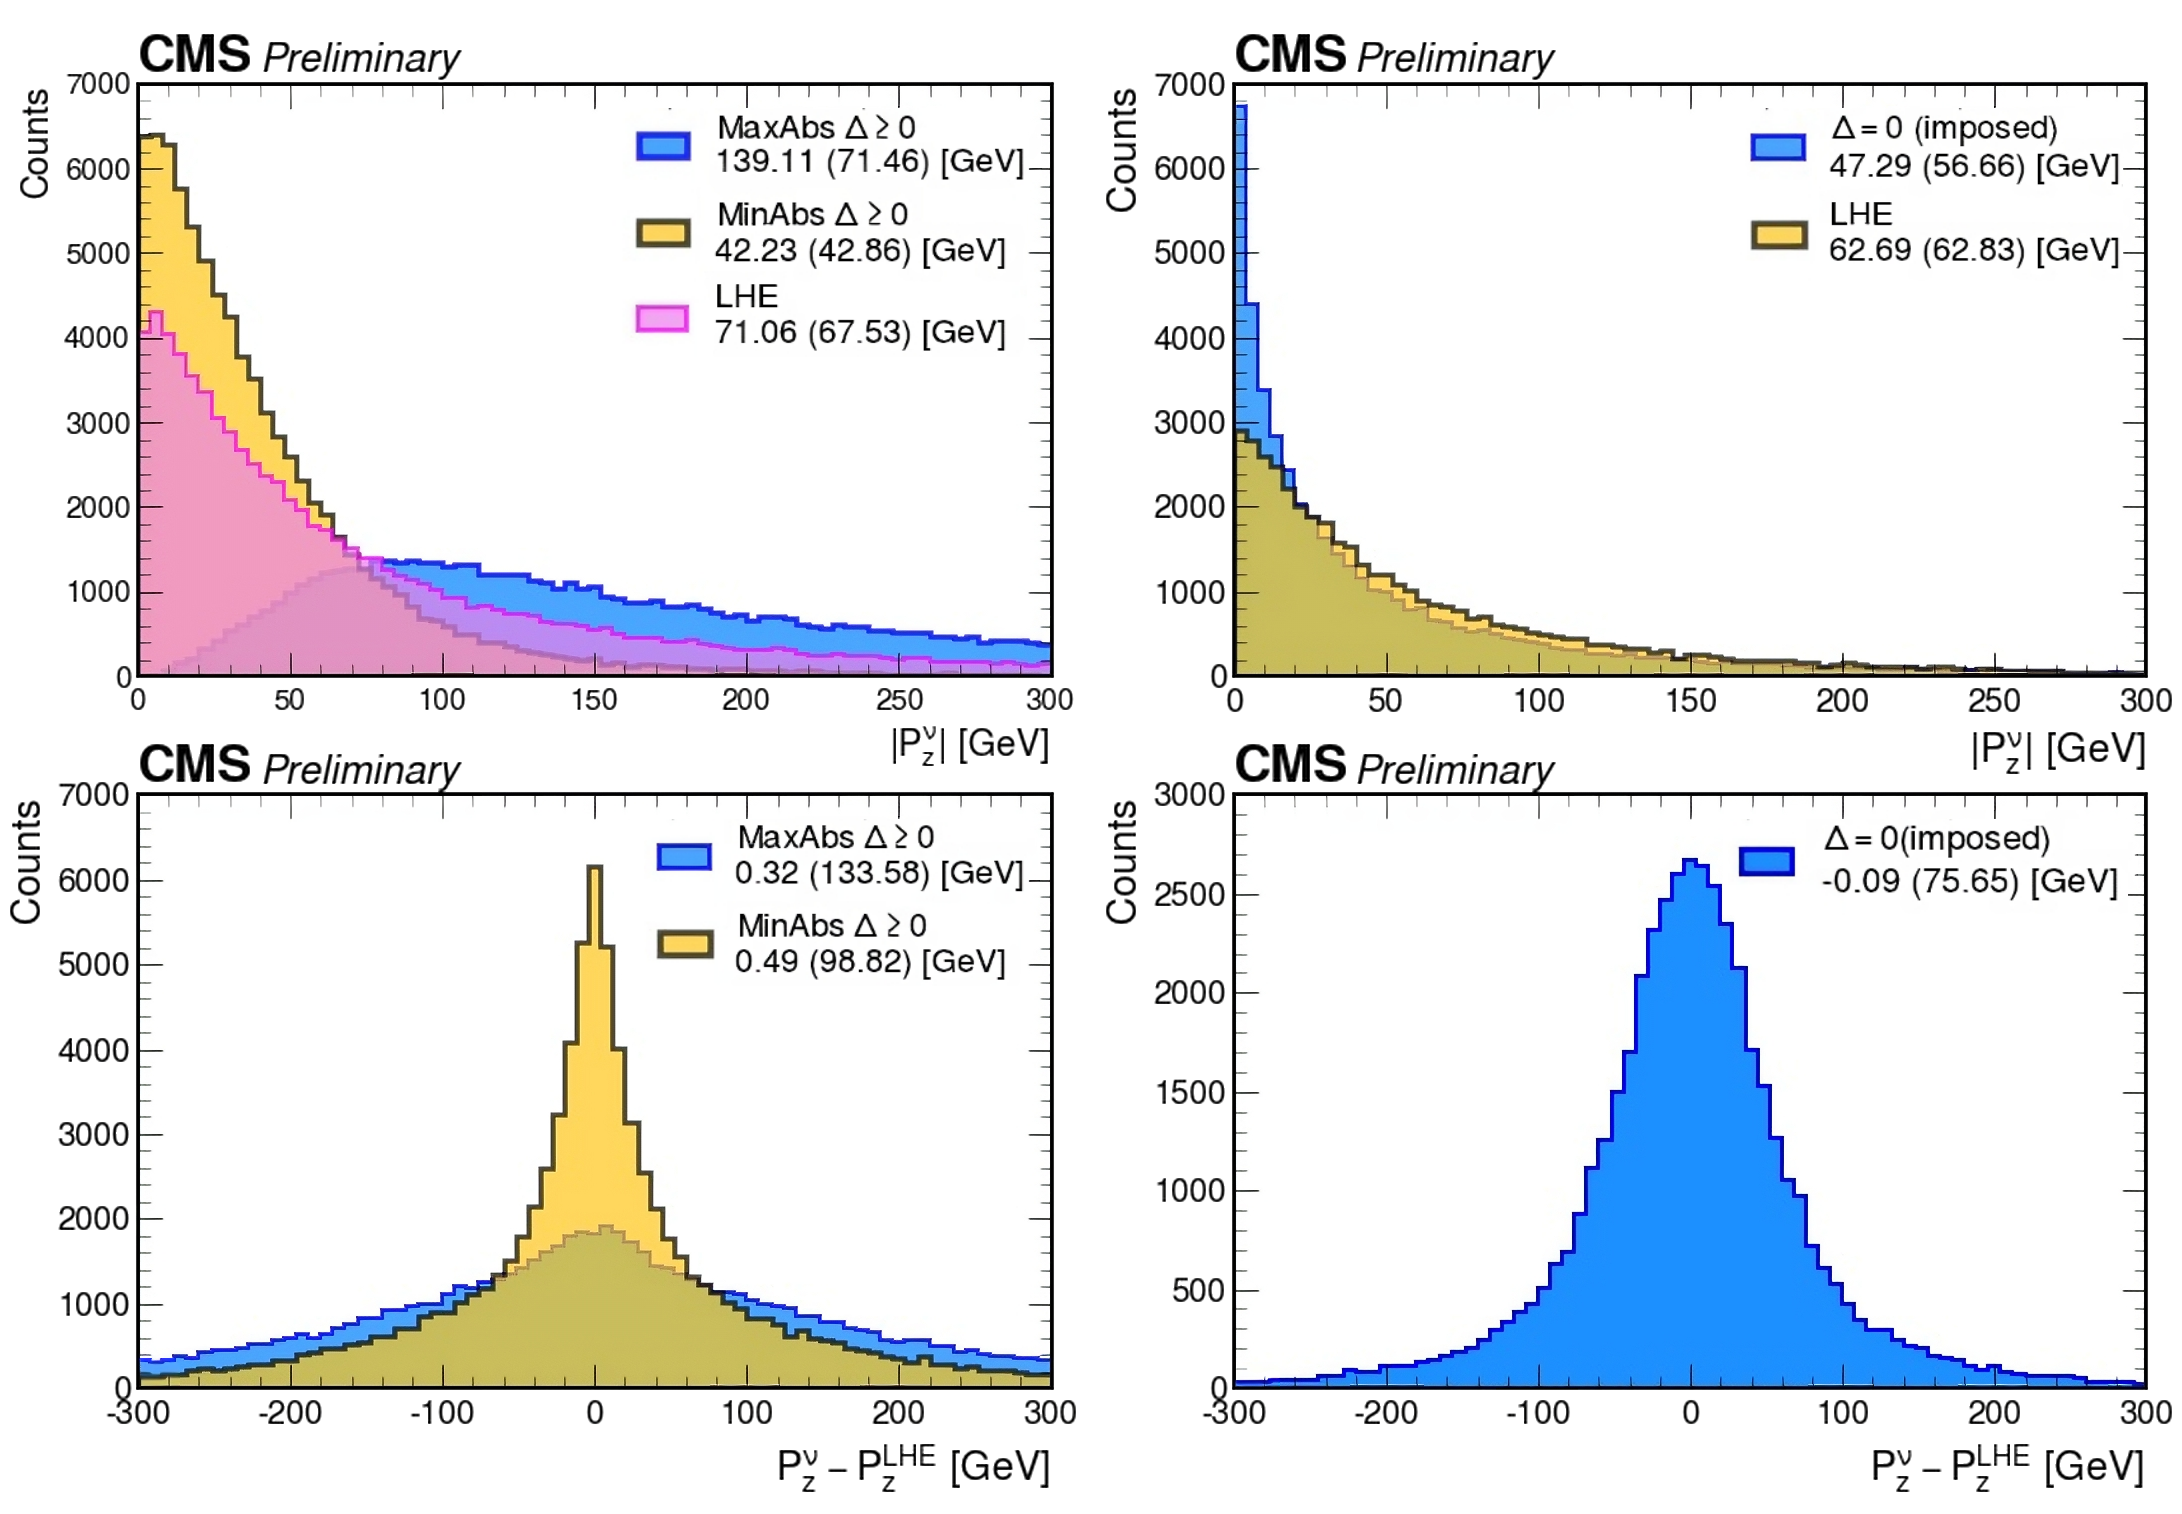
\includegraphics[width=1\linewidth]{fig//chap07-selection/Pznu_LHE_comparison.png}
    \caption{In the left panels there are the events that have two real solutions, while in the right panel the ones with the complex solutions of which only the real part is shown. In the top panel the distribution of the absolute value of the solutions and the LHE truth value are shown, while in the bottom panels, there are the distributions of the differences between the solutions and the LHE truth values. $\Delta$ in the legend is the discriminant of the second order equation. The distributions are in arbitrary units.}
    \label{fig:nu_comparison}
\end{figure}




The distribution of the solutions with the smaller absolute value is in better accordance with the truth value, so the strategy will be:\\
\begin{minipage}{\linewidth}
    \begin{minipage}{0.42\linewidth}

\begin{itemize}
    \item The solution is complex: take the real part.
    \item There are two real solutions: take the smallest in the absolute value.
\end{itemize}

        Of course, in the complex solution case, if we consider only the real part, the chosen value will violate the W mass constraint, so, the invariant mass of the sum of the lepton and the reconstructed neutrino will not be $m_W$. In  \Fig{fig:LeptW_reco} the distribution of the leptonic W mass is shown.
    \end{minipage}
    \hfill
    \begin{minipage}{0.55\linewidth}
    \vspace{-0.2cm}
    \begin{figure}[H]
    \centering
    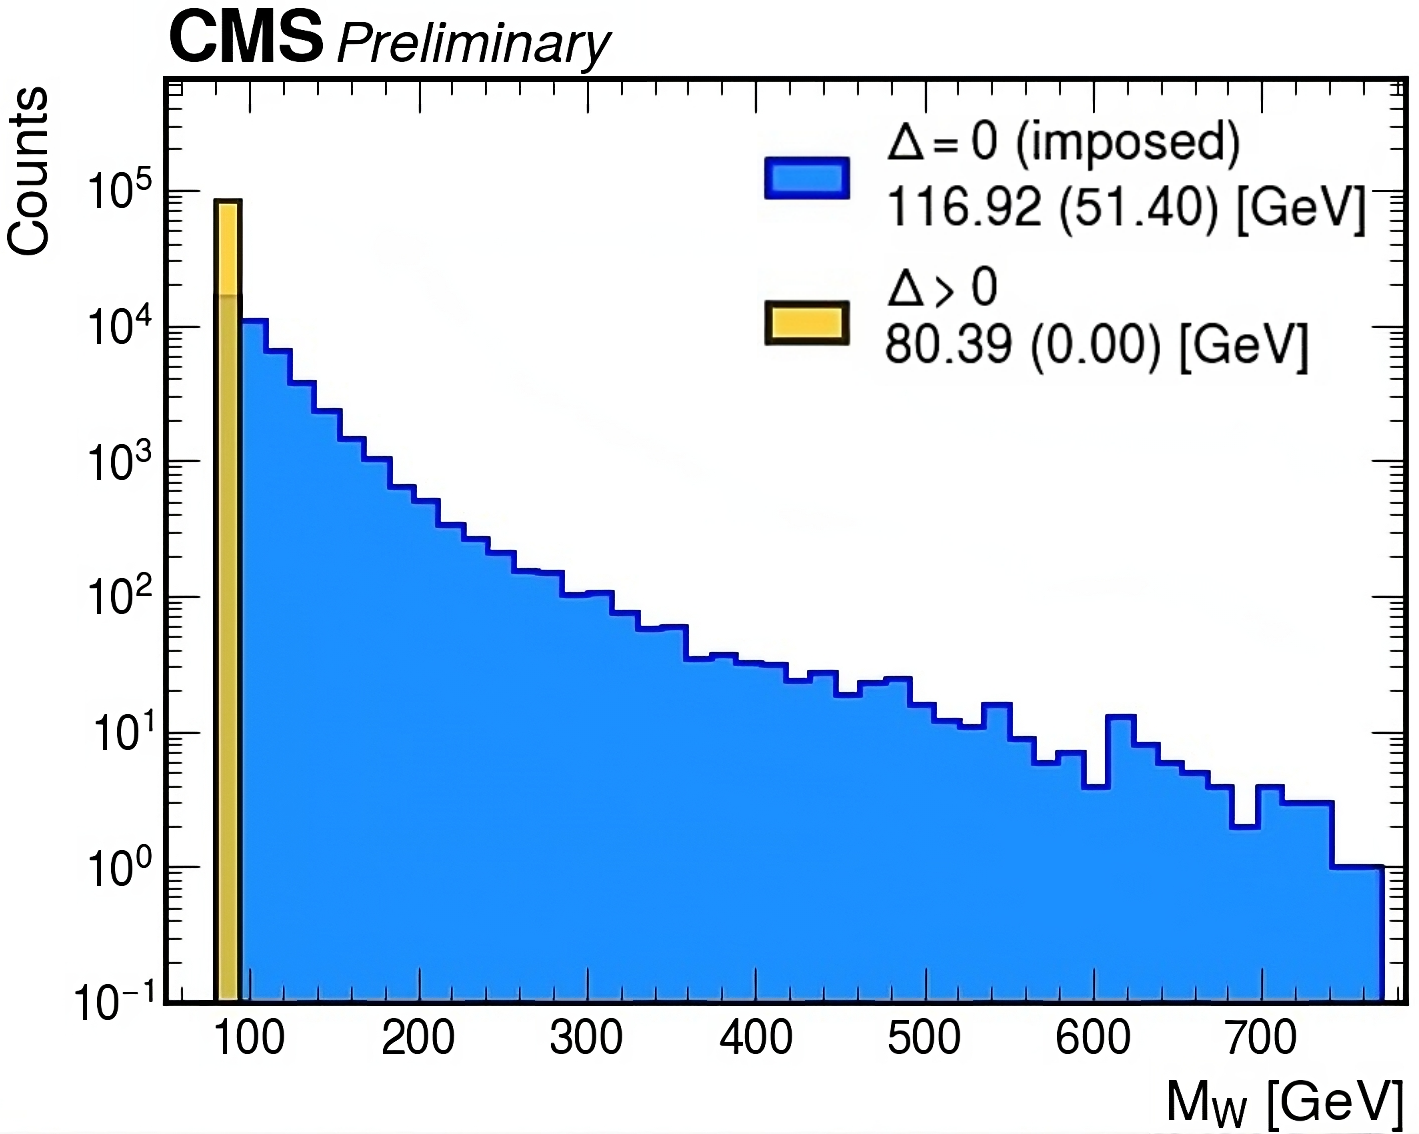
\includegraphics[width=\linewidth]{fig//chap07-selection/Wmass_reconstructed.png}
    \caption{Distribution of the reconstructed W mass in the real solution case and the complex solution case, taking only the real part.}
    \label{fig:LeptW_reco}
\end{figure}
        
    \end{minipage}

\end{minipage}
